\section{Methodology}


% Descripcion del dataset
\subsection{Dataset}
\begin{frame}{Dataset}
    \begin{columns}
        \begin{column}{0.5\textwidth}
            \begin{itemize}
                \item \textbf{Vindr-mammo} Dataset \citef{phamhieuhuyVinDrMammoLargescaleBenchmark}
                \item 5000 digital mammogram examinations containing for each view:
                \begin{itemize}
                    \item BIRADs
                    \item Breast density
                    \item Bounding box of each finding present on the image
                \end{itemize}
                \item 10 classes of pathological findings
            \end{itemize}
        \end{column}

        \begin{column}{0.5\textwidth}
            \begin{figure}
                \centering
                \includegraphics[height=0.5\textheight,keepaspectratio]{imagenes/vista_vindr.png}
                \caption{Example of a mammogram from the Vindr-mammo dataset.}
            \end{figure}
        \end{column}
    \end{columns}
\end{frame}

\begin{frame}{Dataset Distribution}
    
\end{frame}

% Procesamiento de imagenes
\subsection{Image Processing}

\begin{frame}{Image Processing Pipeline}
    \begin{itemize}
        \item Each DICOM Image is normalised to a range of $[0, 1]$
        \item Apply CLAHE algorithm \citef{pizerContrastlimitedAdaptiveHistogram1990} for histogram equalization at 2 different scales
        \item Fuse the equalized images with the original, channel-wise
        \item Image is cropped to the bounding box of the breast using Otsu's thresholding.
    \end{itemize}
\end{frame}

\begin{frame}[plain]
    \begin{figure}
        \centering
        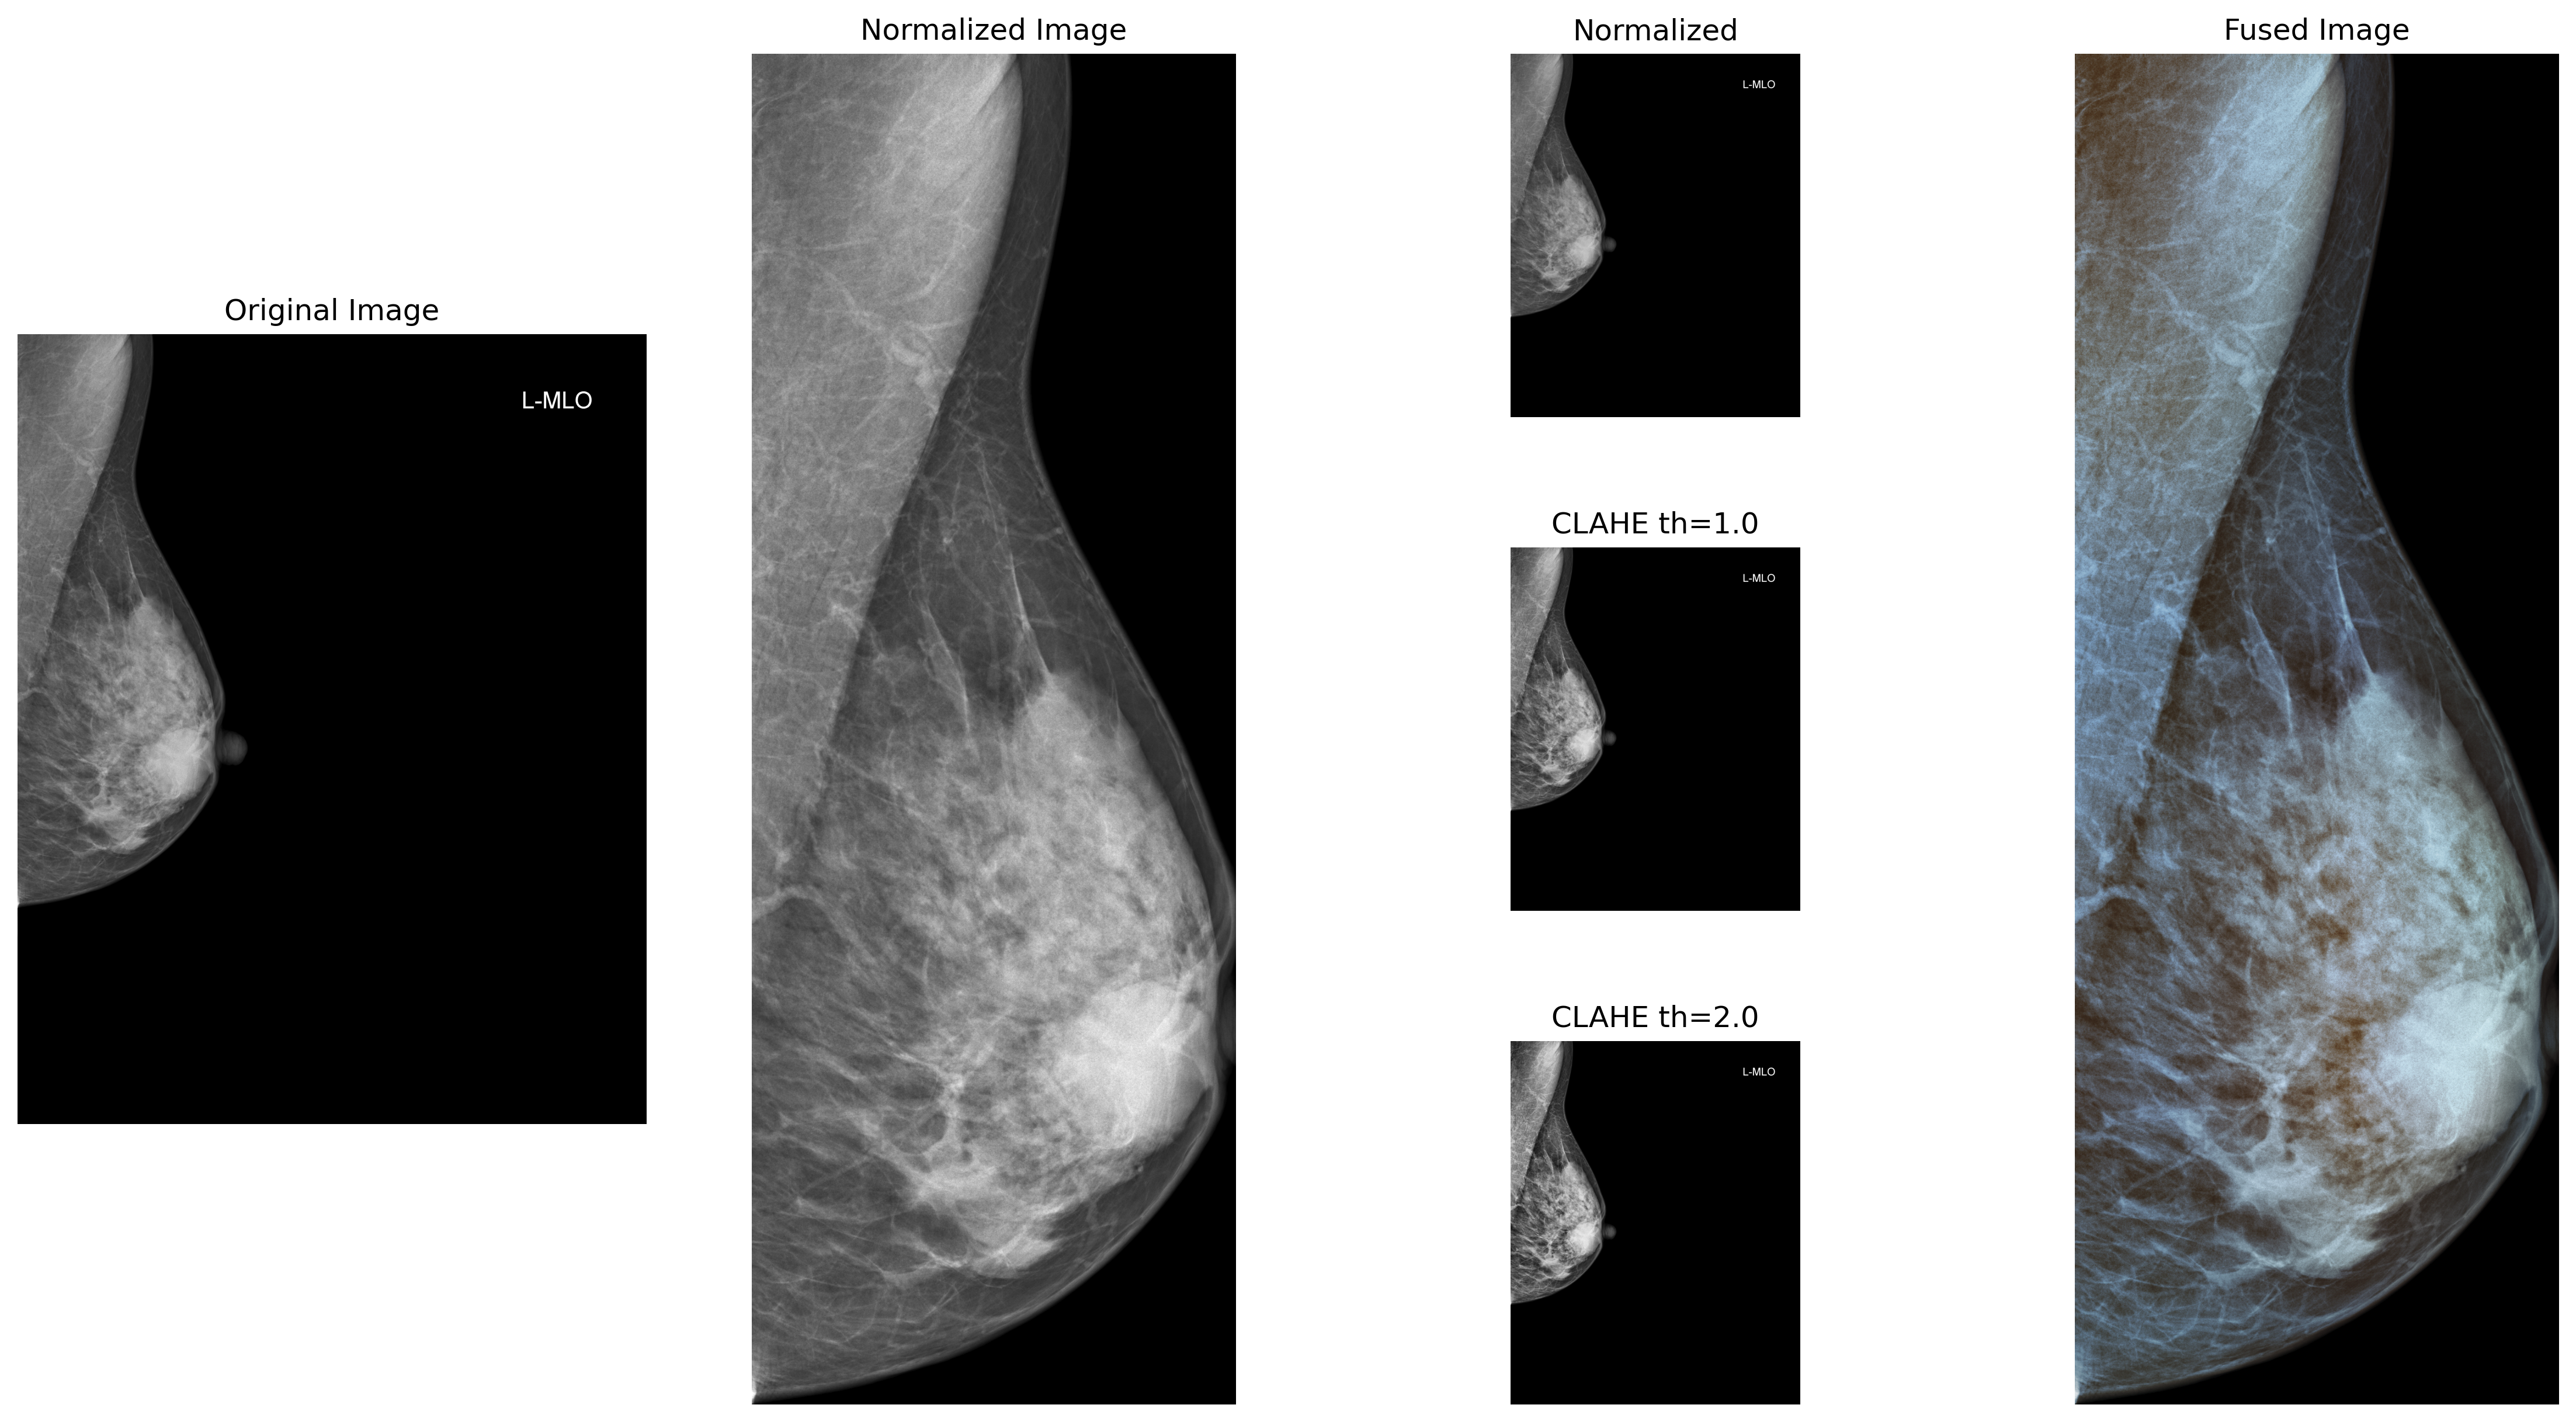
\includegraphics[height=0.9\textheight]{imagenes/improcessingV2.png}
        \caption{Image processing pipeline}
    \end{figure}
\end{frame}
% Seleccion de nuestro modelo
\begin{frame}{Evaluation of deep learning architectures}
    We evaluated the following architectures as a backbone:
    \begin{itemize}
        \item ResNet50
        \item EfficientNetV2
        \item DenseNet
        \item Swin Transformer
        \item MobileNet
        \item VGG19
    \end{itemize}

    Classifier Layer using 2 layer MLP with 512 hidden units and ReLU activation.
    Output layer with 10 units and sigmoid activation.
\end{frame}

% Modelo de extraccion de caracteristicas
\begin{frame}{Feature Extraction Model}
    \begin{itemize}
        \item We use the backbone of the selected architecture as a feature extractor.
        \item The output of the backbone is flattened and fed to the classifier.
        \item The classifier is trained using the cropped images.
    \end{itemize}
\end{frame}





% Analisis mediante ventans

